\documentclass{article}

\PassOptionsToPackage{numbers, sort, compress}{natbib}
\usepackage[main,final]{neurips_2025}

\usepackage[T1]{fontenc}
\usepackage[utf8]{inputenc}
\usepackage{hyperref}
\usepackage{url}
\usepackage{booktabs}
\usepackage{nicefrac}
\usepackage{microtype}
\usepackage{xcolor}

%%%

\usepackage{subcaption}
\usepackage{graphicx}
\usepackage{multirow}
\usepackage{amsmath,amssymb,amsfonts}
\usepackage{amsthm}
\usepackage{mathrsfs}
\usepackage{xcolor}
\usepackage{textcomp}
\usepackage{manyfoot}
\usepackage{algorithm}
%\usepackage{algorithmicx}
\usepackage{algpseudocode}
\usepackage{listings}

\usepackage{wrapfig}

\newtheorem{theorem}{Theorem} % continuous numbers
%%\newtheorem{theorem}{Theorem}[section] % sectionwise numbers
%% optional argument [theorem] produces theorem numbering sequence instead of independent numbers for Proposition
\newtheorem{proposition}[theorem]{Proposition}% 
\newtheorem{lemma}{Lemma}% 
%%\newtheorem{proposition}{Proposition} % to get separate numbers for theorem and proposition etc.

\newtheorem{example}{Example}
\newtheorem{remark}{Remark}

\newtheorem{definition}{Definition}
\newtheorem{assumption}{Assumption}


%%%


\title{Inductive Bias Meta-Learning with Generative Models}


% The \author macro works with any number of authors. There are two commands
% used to separate the names and addresses of multiple authors: \And and \AND.
%
% Using \And between authors leaves it to LaTeX to determine where to break the
% lines. Using \AND forces a line break at that point. So, if LaTeX puts 3 of 4
% authors names on the first line, and the last on the second line, try using
% \AND instead of \And before the third author name.


\author{
  Name Surname\\
  MIPT\\
  Moscow, Russia\\
  \texttt{email@phystech.edu}\\
  \And
  Name Surname\\
  MIPT\\
  Moscow, Russia\\
  \texttt{email@phystech.edu}\\
}


\begin{document}
\raggedbottom 


\maketitle

\begin{abstract}
    This paper investigates inductive bias in machine learning models. By inductive bias we mean the preference of a model for certain types of functions or data structures over others. To analyze the inductive bias of a fixed model, we consider a problem of finding data that this model can fit and generalize on particularly well. Previous work demonstrated that generating labels for a fixed dataset allows one to extract the inductive bias. Here, we extend this approach by proposing a method for generating full synthetic datasets. We train a generative model to produce datasets on which the target model achieves strong generalization performance. We test the proposed framework on CNNs and RNNs, and analyze obtained datasets for each model.
\end{abstract}

\textbf{Keywords:} inductive bias, meta-learning, generative models.

\section{Introduction}\label{sec:intro}

Inductive bias plays a fundamental role in a model’s ability to generalize ~\cite{mitchell1980need}. Without additional assumptions, any hypothesis that fits a finite training dataset is considered equally likely by the model, which can lead to poor generalization. Thus, effective generalization requires a set of prior assumptions about the data, and these assumptions constitute the model’s inductive bias. Understanding and exploiting inductive bias can be a powerful tool for enhancing model performance.

The term “inductive bias” does not have a single, strict definition. For instance, inductive bias can mean underlying assumptions about the domain and task or specific implementation choices that constrain or order the space of hypotheses ~\cite{provost1995inductive}. In this paper, by inductive bias we mean a model's preference for certain types of functions or data structures over others, expressed through better generalization performance. For example, convolutional neural networks (CNNs) are inductively biased towards data with local structure and translation invariance~\cite{726791, wang2024theoreticalanalysisinductivebiases, cohen2017inductivebiasdeepconvolutional}, while recurrent neural networks (RNNs) are inductively biased towards ordered data with sequential structure~\cite{lstm, ishii2023empiricalanalysisinductivebias,DUBININ2024106179}.

A clear understanding of the correspondence between models (or their specific components) and inductive biases is useful for solving machine learning problems. However, this task is highly non-trivial: for most models with complex architecture, the problem of detecting inductive bias is analytically intractable. Several approaches have been developed to extract and characterize the inductive bias of models. Boopathy et al.~\cite{boopathy2024exactcomputationinductivebias} proposed a method to quantify the amount of inductive bias of tasks or models as the amount of information required to specify well-generalizing models within a given hypothesis space. Si et al.~\cite{si2023measuringinductivebiasesincontext} investigated the inductive bias of in-context learning by constructing underspecified demonstrations. Li et al.~\cite{li2021meta} proposed a framework to capture the inductive biases in a learning system by meta-learning Gaussian process kernel hyperparameters from its predictions.

One recent result in this area is the meta-learning framework introduced by Dorrell et al.~\cite{dorrell2023metalearninginductivebiasessimple}, which identifies the inductive bias of differentiable supervised learning algorithms by generating labels for a fixed dataset. For all its strengths, this approach has certain limitations. First, it requires access to input data or its distribution. Second, its analysis of inductive bias is constrained by the fixed dataset and its structure. 

Here, we propose to extend this approach by generating entire synthetic datasets. The meta-learning loop proceeds as follows: an outer generative model, or meta-learner, produces a dataset, which is used to train and test an inner model, or learner, whose inductive bias we aim to extract. After the learner is trained, the quality of its predictions on test data from this dataset is incorporated into the meta-learner's loss function. Thus, the meta-learner learns to generate datasets on which the target model shows the best generalization performance; these are datasets towards which it is inductively biased.

The proposed approach requires no knowledge of the input data distribution, making it more flexible. We expect it to enable a more comprehensive analysis of inductive bias.

\textbf{Contributions.} Our contributions can be summarized as follows:
\begin{itemize}
    \item We present a generative meta-learning framework for extracting the inductive bias of a target model. Unlike prior work~\cite{dorrell2023metalearninginductivebiasessimple} that generates only labels for samples from a fixed distribution, our approach produces entire synthetic datasets via a meta-learned generative model.
    \item We empirically evaluate our algorithm on CNNs and RNNs and compare the results with the known inductive biases of these architectures. For CNNs, we expect to detect a local structure in the generated datasets; for RNNs, we expect them to have a sequential structure.
    \item We highlight the implications of our findings for understanding and leveraging inductive bias. Our method is general-purpose: it can be used to extract inductive bias of any differentiable supervised learning algorithm and, consequently, to improve the generalization performance of models in machine learning problems.
\end{itemize}


\textbf{Outline.} The rest of the paper is organized as follows...

\section{Problem statement}\label{sec:prostate}
We study the problem of extracting and characterizing the inductive bias of learning models by finding the datasets that they generalize best. We now present a formal statement of the problem.

Let \(\mathbb{X} \subset \mathbb{R}^n\) be the input space, \(\mathbb{Y} \subset \mathbb{R}^m\) be the output space and \(\mathbf{f}_{\boldsymbol{\theta}}  : \mathbb{X} \to \mathbb{Y}\) be the target model, where $\boldsymbol{\theta} \in \Theta \subset \mathbb{R}^k$ are its parameters. Let \(\ell(\mathbf{f}_{\boldsymbol{\theta}}(\mathbf{x}), \mathbf{y})\) be the loss function of the target model.

Consider a parametric family of distributions \(p(\mathbf{x} | \mathbf{y}, \mathbf{w})\), where $\mathbf{w} \in \mathbb{W} \subset \mathbb{R}^l$ are the parameters of the distribution. For a fixed label \(\mathbf{y} \in \mathbb{Y}\), a sample \(\mathbf{x} \sim p(\mathbf{x} | \mathbf{y}, \mathbf{w})\) is produced by the generator $\mathbf{g}(\mathbf{w})$.

We aim to find data distribution function \(p^*\), corresponding to parameters \(\mathbf{w}^*\), the solution to the following optimization problem:
\[
\mathbf{w}^* = \arg\min_{\mathbf{w} \in \mathbb{W}} \mathrm{E}_{\mathfrak{D}_{\text{train}}, \mathfrak{D}_{\text{test}} \sim p(\mathbf{x} | \mathbf{y}, \mathbf{w})} \left[ \mathcal{L}\left( \mathbf{f}_{\boldsymbol{\hat{\theta}}}, \mathfrak{D}_{\text{test}} \right) \right] \quad \text{s.t.} \quad |\mathfrak{D}_{\text{train}} \cup \mathfrak{D}_{\text{test}}| = d
\]
where 
\[\boldsymbol{\hat{\theta}} = \arg\min_{\boldsymbol{\theta} \in \Theta}\sum_{(\mathbf{x}, \mathbf{y}) \in \mathfrak{D}_{\text{train}}} \ell(\mathbf{f}_{\boldsymbol{\theta}}(\mathbf{x}), \mathbf{y}).\]
Function \(\mathcal{L}\) measures a model's ability to generalize by calculating the prediction error on a test set and also contains regularization terms to avoid trivial solutions. For example, prediction error can be estimated as cross-entropy or mean squared error (MSE), defined respectively as:
\[
\mathcal{L}_{\text{CE}} = -\frac{1}{|\mathfrak{D}_{\text{test}}|} \sum_{(\mathbf{x}, \mathbf{y}) \in \mathfrak{D}_{\text{test}}} \sum_{i=1}^{m} y_i \log\big( [\mathbf{f}_{\boldsymbol{\hat{\theta}}}(\mathbf{x})]_i \big), \qquad
\mathcal{L}_{\text{MSE}} = \frac{1}{|\mathfrak{D}_{\text{test}}|} \sum_{(\mathbf{x}, \mathbf{y}) \in\mathfrak{D}_{\text{test}}} \| \mathbf{y} - \mathbf{f}_{\boldsymbol{\hat{\theta}}}(\mathbf{x}) \|^2.
\]
The regularization term can be the entropy of the found distribution, defined as:
\[
\mathcal{R}_{\text{ent}}(\mathbf{w}) = - \mathrm{E}_{\mathbf{y}} \left[ \int_{\mathbb{X}} p(\mathbf{x} | \mathbf{y}, \mathbf{w}) \log p(\mathbf{x} | \mathbf{y}, \mathbf{w}) \, d\mathbf{x} \right].
\]

\section{Method}\label{sec:method}
Our proposed approach is to meta-train a generative model to produce datasets on which the target model exhibits the best generalization performance, i.e., datasets to which it is inductively biased. In this section we describe our method in detail.

\begin{wrapfigure}{l}{0.4\textwidth}
    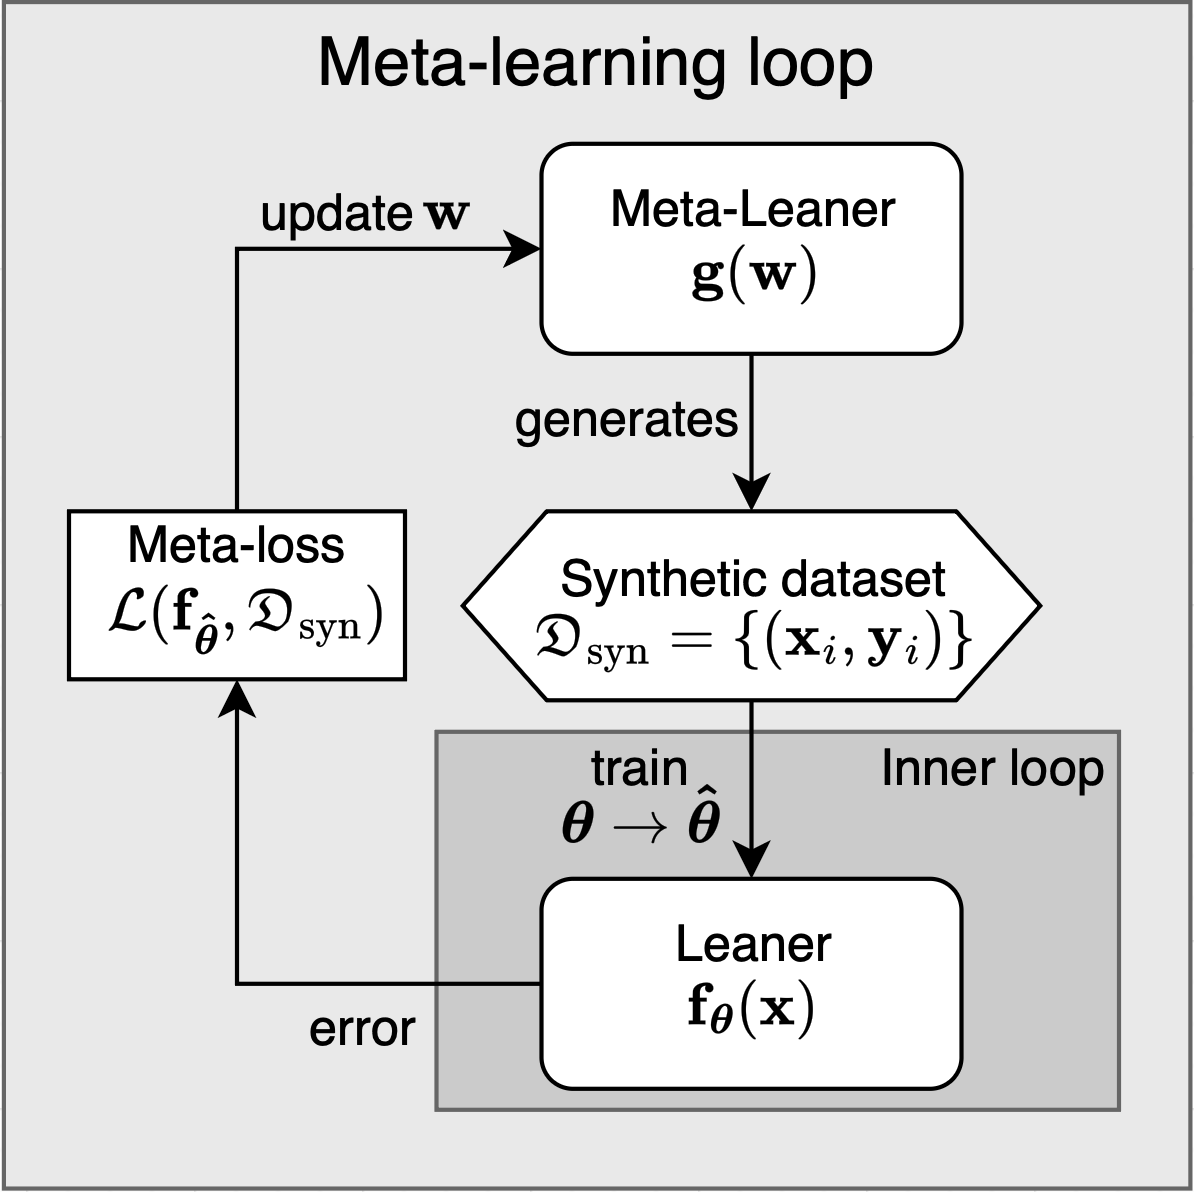
\includegraphics[width=\linewidth]{figures/algorithm.png}
    \caption{Meta-learning loop}
\end{wrapfigure}

The meta-learning cycle is structured as follows. First, the generator $\mathbf{g}(\mathbf{w})$ with current  parameters $\mathbf{w}$ constructs a synthetic dataset $\mathfrak{D}_{\text{syn}}$ according to the predefined configuration: for each class, a fixed number of samples is generated. The number of classes and the number of samples per class are both specified as hyperparameters. Then, the resulting dataset is split into training $\mathfrak{D}_{\text{train}}$ and test $\mathfrak{D}_{\text{test}}$ sets.

Next, the target model $\mathbf{f}_{\boldsymbol{\theta}}$ is trained on the training set $\mathfrak{D}_{\text{train}}$ in the inner loop. It is important that the model be re-initialized from scratch at each meta-learning iteration. At the output of the inner loop we obtain a trained model $\mathbf{f}_{\boldsymbol{\hat\theta}}$.

Next, the meta-loss function is calculated. It consists of two terms. The first term $\mathcal{L}_g$ measures the model's generalization quality, estimated on the test set $\mathfrak{D}_{\text{test}}$. This could be, for example, MSE or Cross-Entropy. The second term $\mathcal{R}$ is the regularization term. Note that if all objects within a class are identical, the target model would easily achieve 100\% accuracy. However, this degenerate case is uninformative. The regularization term is precisely what prevents such trivial solutions. Possible choices include the average distance between objects within the same class, defined as:
\[
\mathcal{R}_{\text{dist}} = \frac{1}{C} \sum_{k=1}^{C} \frac{1}{n_k(n_k - 1)} \sum_{\substack{i,j \in \mathcal{I}_k \\ i \neq j}} \|\mathbf{x}_i - \mathbf{x}_j\|_2^2,
\]
where $C$ is the number of classes in the dataset, $n_k$ is the number of objects in class $k$, and $\mathcal{I}_k$ is the set of indices of objects belonging to class $k$.

Another regularization strategy is to penalize small singular values of the generator's weight matrix, as this helps to avoid degeneracy. The corresponding regularization term is defined as:
\[
\mathcal{R}_{\text{svd}} = \frac{1}{r} \sum_{k=1}^{r} \bigl(\max(\tau - \sigma_k, 0)\bigr)^2,
\]
where $\sigma_1, \dots, \sigma_r$ are the singular values of the weight matrix and $\tau$ is a fixed threshold.

Thus, during meta-training, the meta-loss is minimized by updating the generator parameters $\mathbf{w}$, resulting in a generator $\mathbf{g}(\mathbf{\hat w})$ that produces datasets which are easy for the target model to generalize from. The structure of these datasets reflects the model's inductive bias.

The proposed meta-learning procedure is summarized in Algorithm \ref{alg:meta_learning}.

\begin{algorithm}[H]
\caption{Meta-learning for inductive bias extraction}
\label{alg:meta_learning}
\begin{algorithmic}[1]
\State Initialize generator $\mathbf{g}(\mathbf{w})$ with random parameters $\mathbf{w}$
\While{step $<$ total steps}
    \State Generate synthetic dataset $\mathfrak{D}_{\text{syn}} = \{(\mathbf{x}_i, \mathbf{y}_i)\}$ with $C$ classes and $N$ samples per class
    \State Split $\mathfrak{D}_{\text{syn}}$ into training set $\mathfrak{D}_{\text{train}}$ and test set $\mathfrak{D}_{\text{test}}$
    \State Re-initialize target model $\mathbf{f}_{\boldsymbol{\theta}}$ from scratch
    \State Train $\mathbf{f}_{\boldsymbol{\theta}}$ on $\mathfrak{D}_{\text{train}}$ in the inner loop $\rightarrow$ trained model $\mathbf{f}_{\boldsymbol{\hat\theta}}$
    \State Compute meta-loss: $\mathcal{L}_{\text{meta}} = \mathcal{L}_g(\mathbf{f}_{\boldsymbol{\hat\theta}}, \mathfrak{D}_{\text{test}}) + \lambda \mathcal{R}(\mathfrak{D}_{\text{syn}})$
    \State Take $\mathbf{w}$ gradient step on meta-loss
\EndWhile
\end{algorithmic}
\end{algorithm}
Similar to previous work~\cite{dorrell2023metalearninginductivebiasessimple}, our approach can be extended to compare the inductive biases of two models, i.e., to find a dataset that is easy for one model to generalize from but difficult for the other. In this case, both models are trained in the inner loop, and the measure of the generalization quality of the second model is subtracted when computing the meta-loss. Consequently, minimizing this meta-loss improves the generalization of the first model while degrading that of the second.

\section{Experiments}\label{sec:exp}

\subsection{Baseline experiment}

First, we replicate the experiment by Dorell et al.~\cite{dorrell2023metalearninginductivebiasessimple} on extracting inductive bias via label generation. Their algorithm proceeds as follows: the meta-learner generates labels for a dataset, which is subsequently used to train the learner; the learner's generalization performance on these labels is then evaluated and incorporated into the meta-loss function. In this way, the meta-learner is trained to find functions that the learner can easily generalize.

As the target model, we use linear regression, and as the meta-learner, a 4-layer MLP. The meta-loss function consists of three terms: the MSE of the linear regression on the test set, the Sinkhorn distance of the label distribution from a uniform distribution, and terms that account for previously obtained functions to ensure orthogonality with them.

As a result of the experiment, we obtained three orthogonal linear functions, as expected.

\subsection{Proposed Framework Evaluation}

To empirically validate our algorithm, we conducted computational experiments to extract the inductive bias of CNNs and RNNs. Specifically, we verify that the generative model learns to create datasets on which the target model shows the best generalization performance, investigate the influence of different regularization terms on the generated data, and attempt to interpret the obtained results in light of the well-known inductive biases of these architectures.

Data in our experiments is fully synthetic. For CNNs we generate datasets of images with a given number of classes and number of objects per class. As a generative model, we used a variational autoencoder (VAE) decoder. It transforms a vector from a latent space, consisting of class embedding and random noise sampled from a standard normal distribution \(\mathcal{N}(0, 1)\), into a grayscale image.

The meta-learning process is implemented using the learn2learn library~\cite{arnold2020learn2learnlibrarymetalearningresearch}. Specifically, to enable end-to-end differentiability, we wrap the inner learner in a MAML (Model-Agnostic Meta-Learning)~\cite{finn2017modelagnosticmetalearningfastadaptation} wrapper. This allows us to clone the learner for each meta-step, train it on the generated dataset, and still keep the computational graph needed to propagate gradients from the meta-loss back to the generator. We use Adam~\cite{kingma2017adammethodstochasticoptimization} as the optimizer for meta-learning.

As measures of generalization performance, we use MSE and cross-entropy and then compare them. We also conduct a comparative analysis of different types of regularization terms: the entropy of the distribution, the average distance between objects of the same class, and the singular values of the generator's weight matrix.

List of expected figures:
\begin{itemize}
    \item graph comparing different types of regulation (x-axis - meta-iterations, y-axis - accuracy, \%);
    \item figure with examples of the resulting datasets;
    \item meta-loss change chart (x-axis - meta-iterations, y-axis - meta-loss).
\end{itemize}

\subsection{CNNs and 1×4 Images}
We first test our method on a simple example: CNNs with a 1×2 convolution and 1×4 images. As a generator, we use a trainable tensor, meaning that the elements of the synthetic dataset are directly optimized as parameters. For the meta-learning process, we wrap the CNN in a MAML (Model-Agnostic Meta-Learning) wrapper~\cite{finn2017modelagnosticmetalearningfastadaptation} from the learn2learn library~\cite{arnold2020learn2learnlibrarymetalearningresearch}. For the outer loop, we use the Adam optimizer~\cite{kingma2017adammethodstochasticoptimization}.

The CNN architecture is as follows: a convolution with a 1×2 kernel and stride (1,2), followed by max pooling, and finally a linear layer that outputs class logits. In the experiment we uses the following parameters: 2 classes, 20 samples per class, 5 inner loop steps, and learning rates of 0.5 and 0.01 for inner and outer loop 
respectively. As a measure of prediction error on the test set, we use MSE. For regularization, we experiment with two terms: the mean intra-class distance and a penalty on small singular values of the data matrix computed via SVD.

\begin{figure}[H]
    \centering
    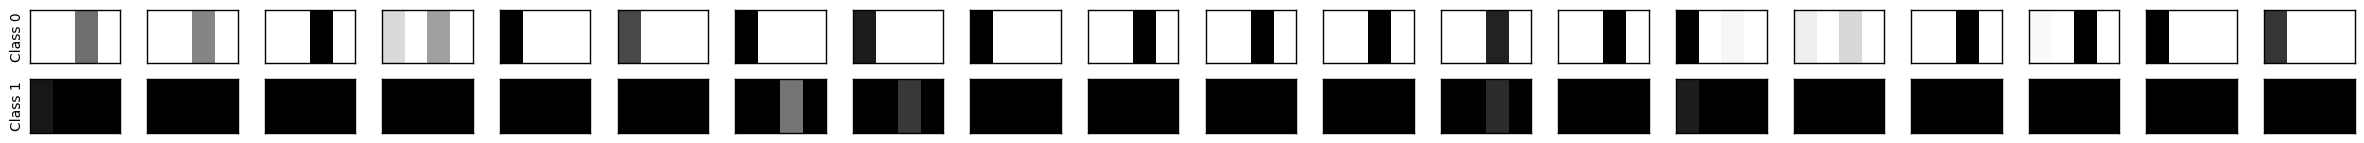
\includegraphics[width=1\textwidth]{figures/CNN_1x4/1x4_without_reg.png}
    \caption{Obtained dataset without regularization}
    \label{fig:1x4_without_reg}
\end{figure}

\begin{figure}[H]
    \centering
    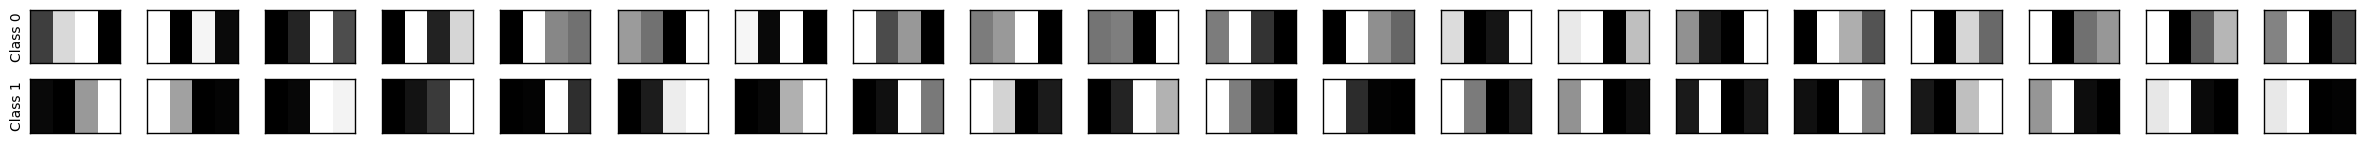
\includegraphics[width=1\textwidth]{figures/CNN_1x4/1x4_class_diversity.png}
    \caption{Obtained dataset with class diversity regularization}
    \label{fig:1x4_class_diversity}
\end{figure}

\begin{figure}[H]
    \centering
    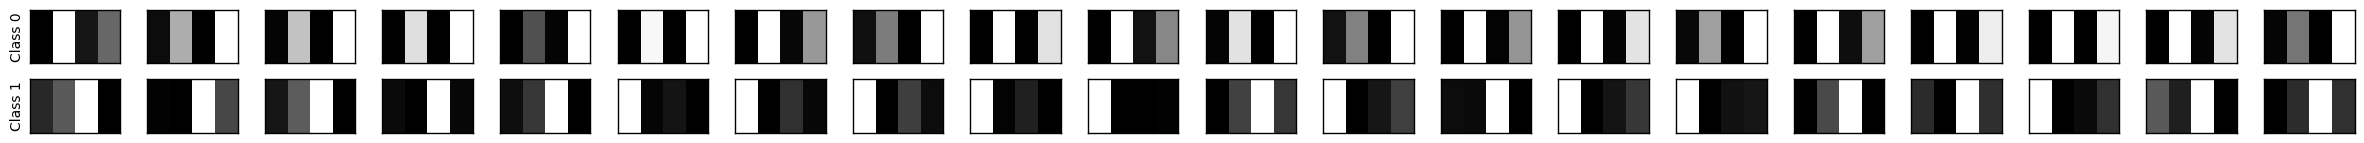
\includegraphics[width=1\textwidth]{figures/CNN_1x4/1x4_svd.png}
    \caption{Obtained dataset with SVD regularization}
    \label{fig:1x4_svd}
\end{figure}

As can be seen, even without regularization, the trivial solution — where all images within a class are identical — does not fully occur. This reveals the convolutional architecture's inductive bias towards locality: within a given class, we observe images where the first and second pairs of pixels are swapped. This indicates that for this architecture, local structure matters more than global structure.

Adding the mean intra-class distance as a regularization term makes the classes more diverse while preserving locality. In class 1, the defining pattern is two black pixels in one of the two positions, while the other position can contain anything — two white pixels, one white and one black, or vice versa. Moreover, the two black pixels may appear either in the left or the right pair. This reflects the inductive bias towards locality: the label is determined by the local structure rather than the global one. The effect of stride (1,2) is also noticeable — class 0 contains an element with two black pixels in the middle, but this does not cause it to be misclassified as class 1.

When penalizing small singular values, the situation is similar — here, the distinguishing pattern for class 0 consists of a black pixel followed by a white pixel, in that exact order.

Thus, the structure of the obtained datasets reflects the inductive bias of CNNs toward data with local structure, which is consistent with previously known results.

\begin{figure}[H]
    \centering
    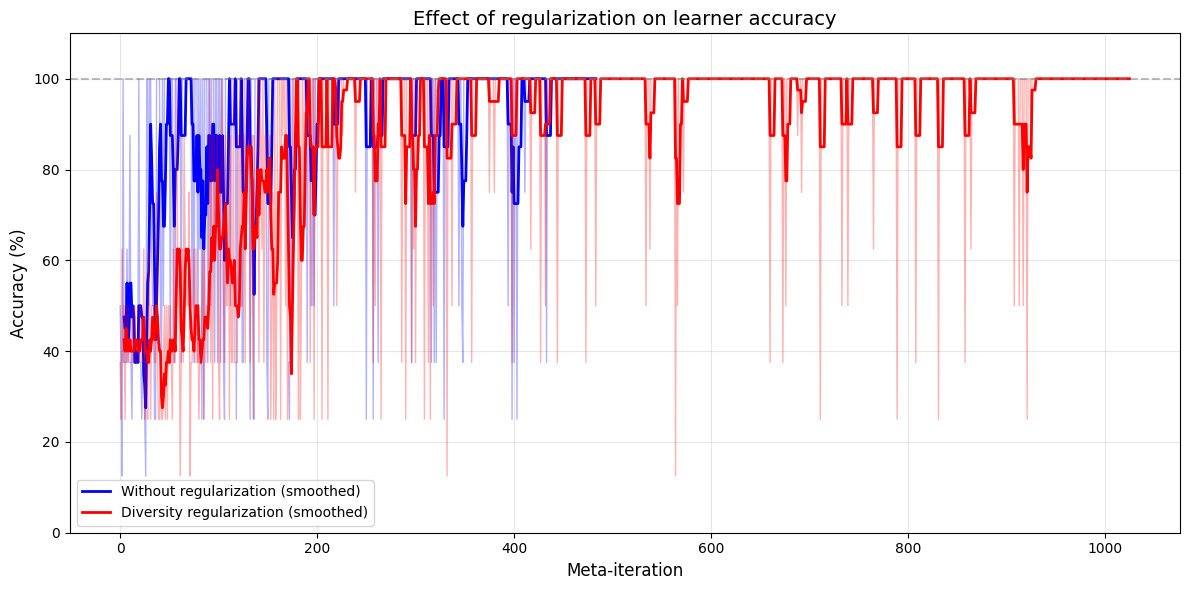
\includegraphics[width=0.8\textwidth]{figures/CNN_1x4/1x4_comparison.png}
    \caption{Comparison of different regularization strategies}
    \label{fig:1x4_comparison}
\end{figure}

\subsection{CNNs and 4x4 images}
Next, we conduct an experiment with CNNs on 4×4 images. As a generator, we again use a trainable tensor. The CNN consists of a single convolutional layer with a 2×2 kernel and stride 2, which reduces a 4×4 input to 4 feature maps of size 2×2. This is followed by ReLU activation and 2×2 max pooling, resulting in 4 feature maps of size 1×1. After flattening, a fully connected layer maps the 4 features to the output classes.

The experimental parameters are as follows: 4 classes, 20 samples per class, 10 inner loop steps, and learning rates of 0.5 and 0.01 for the inner and outer loops, respectively. As the meta-loss function, we use cross-entropy. For regularization, we use the average intra-class distance with a regularization parameter $\lambda = 1.5$.

\begin{figure}[H]
    \centering
    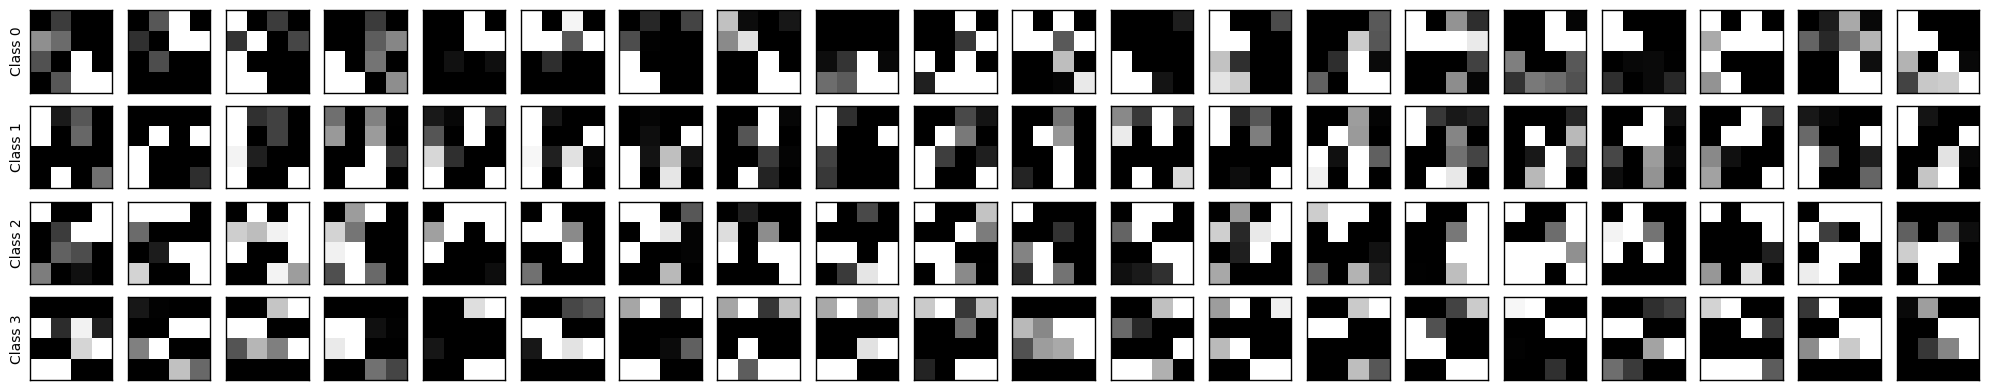
\includegraphics[width=1\textwidth]{figures/CNN_4x4/4x4_dataset.png}
    \caption{Obtained dataset}
    \label{fig:4x4_dataset}
\end{figure}

The obtained dataset is presented on figure \ref{fig:4x4_dataset}.

\begin{figure}[H]
    \centering
    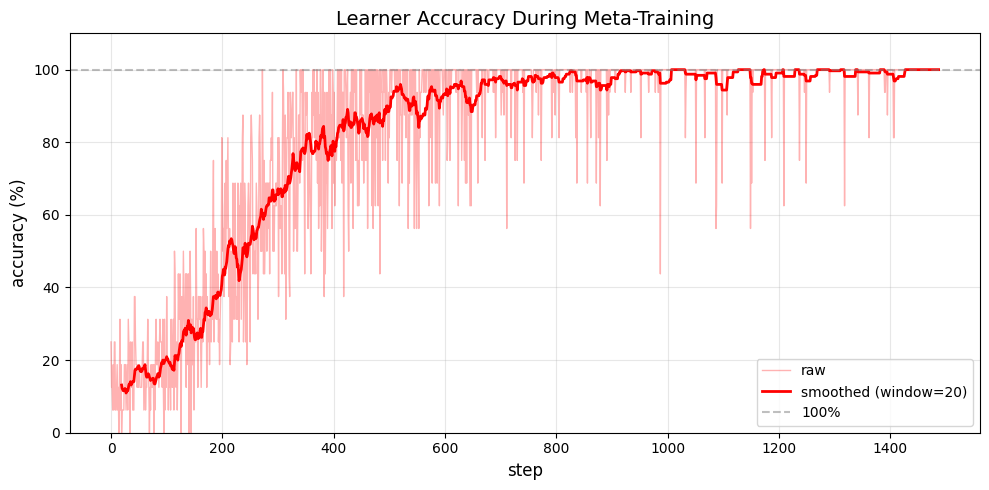
\includegraphics[width=0.8\textwidth]{figures/CNN_4x4/4x4_accuracy.png}
    \caption{Accuracy dependence on meta-iteration}
    \label{fig:4x4_accuracy}
\end{figure}

To characterize the properties of the obtained datasets, we carry out additional analysis to verify the locality of the obtained dataset. First, we train the target model on the original dataset and then validate it on a shuffled dataset, where the $2 \times 2$ blocks within each image are randomly permuted.

\begin{figure}[H]
    \centering
    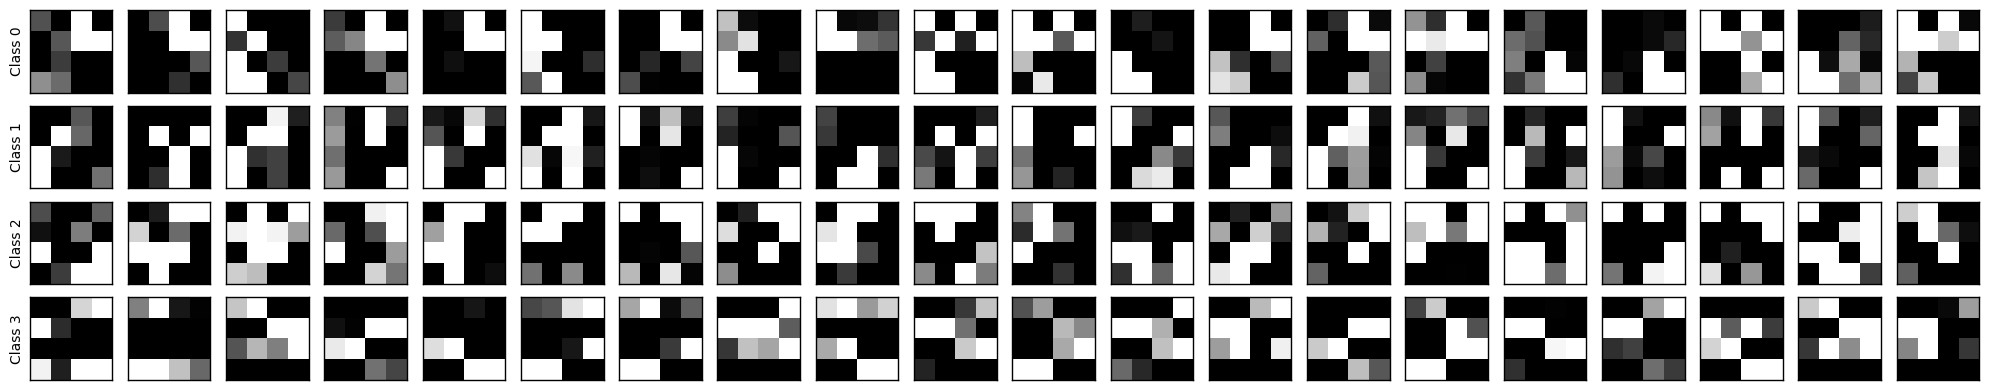
\includegraphics[width=1\textwidth]{figures/CNN_4x4/4x4_shuffled_dataset_42.png}
    \caption{Example of shuffled dataset: seed = 42}
    \label{fig:4x4_shuffled_dataset_42}
\end{figure}

\begin{figure}[H]
    \centering
    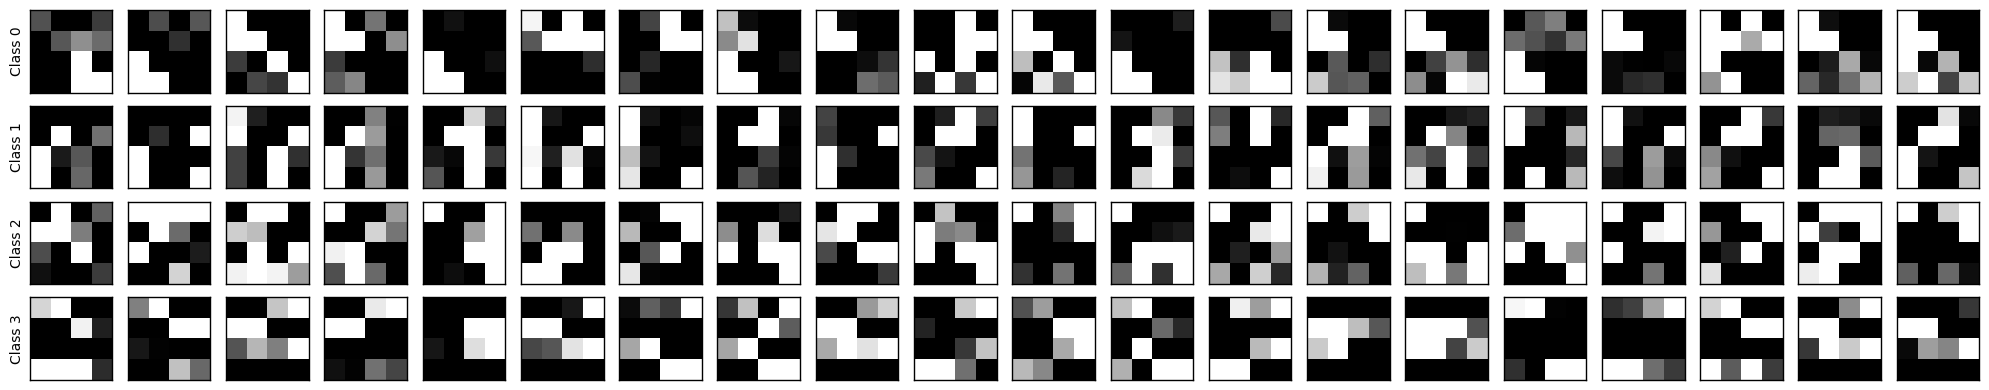
\includegraphics[width=1\textwidth]{figures/CNN_4x4/4x4_shuffled_dataset_123.png}
    \caption{Example of shuffled dataset: seed = 123}
    \label{fig:4x4_shuffled_dataset_123}
\end{figure}

Averaging the results over different splits of the original dataset into training and test sets and over different seeds for shuffling yields the following values:

\begin{table}[h!]
\centering
\begin{tabular}{l c}
\hline
\textbf{Data type} & \textbf{Accuracy (\%)} \\
\hline
Original           & $99.69 \pm 2.56$ \\
Seed 42            & $99.65 \pm 2.53$ \\
Seed 123           & $99.65 \pm 2.53$ \\
Seed 456           & $99.65 \pm 2.53$ \\
Seed 789           & $99.65 \pm 2.53$ \\
\hline
\end{tabular}
\end{table}

As can be seen, the model performs well even on the shuffled dataset. This indicates locality: the model relies on the local structure within $2 \times 2$ blocks rather than on their global arrangement.

We perform a similar experiment, this time training the model on the shuffled dataset and validating it on the original one:

\begin{table}[h!]
\centering
\begin{tabular}{l c}
\hline
\textbf{Data type} & \textbf{Accuracy (\%)} \\
\hline
Shuffled (train)   & $99.00 \pm 5.57$ \\
Original (test)    & $99.24 \pm 3.85$ \\
\hline
\end{tabular}
\end{table}

Again, the values are very close to $100\%$.

Next, we compare our CNN with an MLP, a model that has no explicit inductive bias toward locality and is sensitive to global structure. We conduct the same experiment as for the CNN: training on the original dataset and validating on the shuffled one. The averaged results are as follows:

\begin{table}[h!]
\centering
\begin{tabular}{l c}
\hline
\textbf{Data type} & \textbf{Accuracy (\%)} \\
\hline
Original           & $55.31 \pm 15.52$ \\
Seed 42            & $76.21 \pm 8.55$ \\
Seed 123           & $76.88 \pm 9.16$ \\
Seed 456           & $77.49 \pm 8.53$ \\
Seed 789           & $76.35 \pm 7.67$ \\
\hline
\end{tabular}
\end{table}

This experiment was conducted under the same inner loop parameters as those used for the CNN.

These results confirm the local structure of the data in our dataset, which aligns with the known inductive bias of CNNs. Thus, our method demonstrates strong performance on CNNs.

\subsection{RNNs}
Now we conduct an experiment with  RNNs. As before, we use a trainable tensor as the generator. The architecture of the target model is as follows: the RNN consists of two recurrent layers, each with a hidden dimension of 32. It takes one-hot encoded sequences as input and uses the final hidden state for classification via a linear layer.

The experimental parameters are as follows: 5 classes, 10 samples per class, each sample consisting of 20 letters of the English alphabet encoded as one-hot vectors. The inner loop has 10 steps, with learning rates of 0.5 and 0.01 for the inner and outer loops, respectively. We use MSE as the meta-loss function and the average intra-class distance as regularization, with a regularization parameter $\lambda = 0.1$.

\begin{figure}[H]
    \centering
    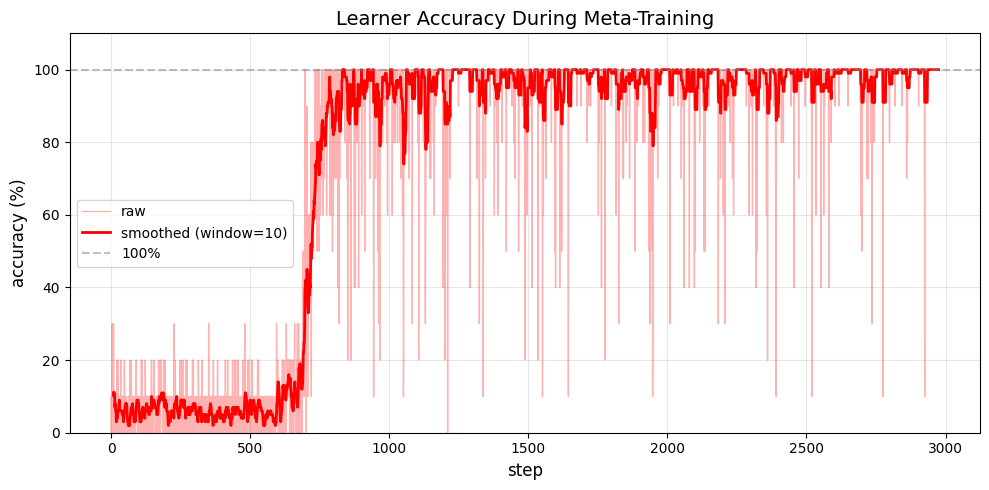
\includegraphics[width=0.8\textwidth]{figures/RNN/accuracy.png}
    \caption{Accuracy dependence on meta-iteration}
    \label{fig:rnn_accuracy}
\end{figure}

Below are five example sequences from each class:

\begin{figure}[H]
    \centering
    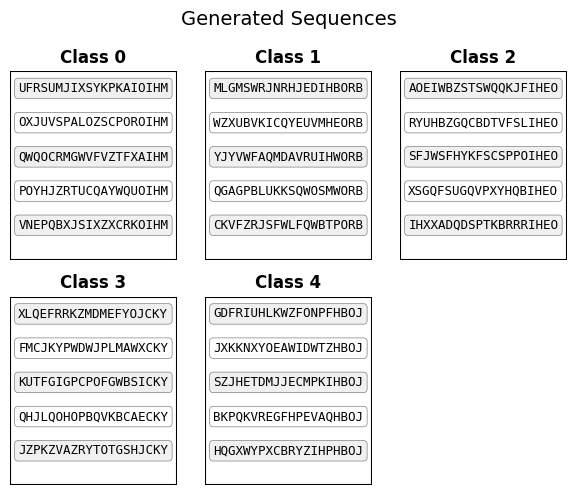
\includegraphics[width=0.5\textwidth]{figures/RNN/dataset_examples.png}
    \caption{Examples of the obtained dataset}
    \label{fig:rnn_dataset}
\end{figure}

We now verify the sequential structure of the obtained dataset. To this end, we train the model on the original dataset and then validate it on the reversed test set. Averaging over different splits of the dataset into training and test sets yields the following results:

\begin{table}[h!]
\centering
\begin{tabular}{l c}
\hline
\textbf{Data type} & \textbf{Accuracy (\%)} \\
\hline
Original           & $100.00 \pm 0.00$ \\
Reversed           & $32.40 \pm 14.08$ \\
\hline
\end{tabular}
\end{table}

We also perform a similar experiment, this time training on the reversed dataset and validating on the original one. The results are shown below:

\begin{table}[h!]
\centering
\begin{tabular}{l c}
\hline
\textbf{Data type} & \textbf{Accuracy (\%)} \\
\hline
Reversed (train)   & $42.20 \pm 27.91$ \\
Original (test)    & $29.10 \pm 17.33$ \\
\hline
\end{tabular}
\end{table}

As can be observed, in both cases, generalization performance drops significantly, indicating that the order of letters plays a crucial role. This confirms the sequential structure of the data. Notably, this aligns with the well-known inductive bias of RNNs, demonstrating that our method works correctly.


\section{Discussion}\label{sec:disc}


\section{Conclusion}\label{sec:concl}



%%%%%%%%%%%%%%%%%%%%%%%%%%%%%%%%%%%%%%%%%%%%%%%%%%%%%%%%%%%%

\bibliographystyle{unsrtnat}
\bibliography{references}

%%%%%%%%%%%%%%%%%%%%%%%%%%%%%%%%%%%%%%%%%%%%%%%%%%%%%%%%%%%%

\newpage
\appendix
\section{Appendix / supplemental material}\label{app}

\subsection{Additional experiments / Proofs of Theorems}\label{app:exp}

TODO

\end{document}
